\subsection{System design}
\label{section:system-design}
Our main system design goals were to make the system extensible and maintainable. That is, adding new features and replacing current implementations should be easy to do, and you should be able to trust that the system works once the change is made.

\subsubsection{Bridge and repository design patterns}
We've tried to achieve this by using the repository and bridge design patterns when possible, particularly to communicate with our database. The repository pattern is used to collect all our database queries in one place, and the bridge pattern is used to abstract away the implementation. Rather than talking directly to the database, our controllers communicate via an interface that defines which operations can be made. For an example of this, see the \inlinecode{IUserRepository} interface \cite{repo:user-repository-interface}.

Because we depend on the abstraction rather than the implementation, we can easily replace the database with a NoSQL database, create a wrapper that does extra operations on top, or similar---and the code depending on the interface won't have to change.

\subsubsection{Object-relational mapping}
In the same spirit as above, we've used GORM \cite{gorm} for object-relational mapping. With this ORM, the database provider is abstracted away, making it possible to replace the database provider without changing the ORM code.

\subsubsection{Separate frontend}
We moved the frontend code to a separate project \cite{repo:frontend}. This way, the Go server has only a single responsibility. This also serves as a way of using the bridge pattern to add another layer of abstraction, because the frontend is now only dependent on the API and not the Go implementation. This would also allow for different frontends to be implemented, like you obtain with MVC.

\subsubsection{Program modules}
In order to improve the single-responsibility aspect of our code, we've used modules to separate code into units of single responsibility as shown in \autoref{table:gomodules}. \autoref{fig:package-relations} shows how these packages are used by each other.
\begin{table}[H]
  \centering
  \begin{tabular}{ll}
    \toprule
    \textbf{Package} & \textbf{Responsibility} \\
    \midrule
    \inlinecode{controllers} & Managing the API routes and implementing the controllers \\
    \inlinecode{database} & Communicate with the database \\
    \inlinecode{internal} & Logging output destination and format --- and error handling \\
    \inlinecode{models} & Model definitions \\
    \inlinecode{monitoring} & Managing Prometheus and monitoring \\
    \inlinecode{password} & Password hashing and validation \\
    \inlinecode{test/controllers} & Integration and unit tests for all controllers \\
    \inlinecode{main} & Starting the application \\
    \bottomrule
  \end{tabular}
  \caption{The packages in our Go server and their responsibilities.}
  \label{table:gomodules}
\end{table}
\begin{figure}[H]
  \centering
  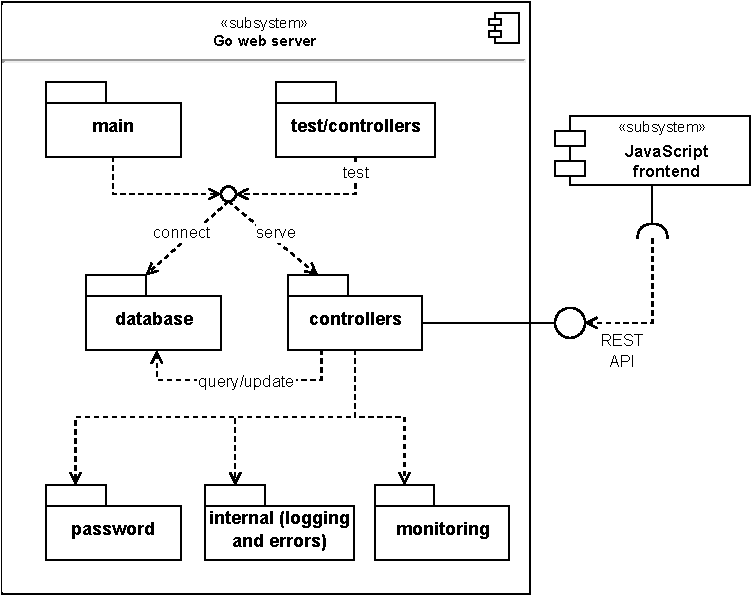
\includegraphics[width=0.85\textwidth]{package-relations/package-relations.pdf}
  \caption{A UML diagram showing how our packages and self-coded subsystems are related.}
  \label{fig:package-relations}
\end{figure}
